% =============================================================================
%  Machine Learning for Petroleum Engineers Using Python
%  Módulo 3 · Clase 2: Clasificación --- Regresión Logística
%  SLB Ecuador | UDLA
%
%  Compilar: pdflatex -shell-escape presentacion.tex (x2 para refs)
% =============================================================================
\documentclass[aspectratio=169, 11pt]{beamer}

% ── Codificación y lenguaje ──────────────────────────────────────────────────
\usepackage[T1]{fontenc}
\usepackage[utf8]{inputenc}
\usepackage[spanish,es-noshorthands]{babel}

% ── Fuentes ──────────────────────────────────────────────────────────────────
\usepackage{FiraSans}
\usepackage{FiraMono}
\renewcommand{\familydefault}{\sfdefault}

% ── Gráficos y diagramas ────────────────────────────────────────────────────
\usepackage{graphicx}
\usepackage{tikz}
\usetikzlibrary{arrows.meta, positioning, shapes.geometric, calc, fit, decorations.pathreplacing}
\usepackage{fontawesome5}

% ── Código fuente ────────────────────────────────────────────────────────────
\usepackage{minted}
\usepackage{tcolorbox}
\tcbuselibrary{minted, skins, breakable}

% ── Tablas y utilidades ──────────────────────────────────────────────────────
\usepackage{amsmath}
\usepackage{colortbl}
\usepackage{booktabs}
\usepackage{multicol}
\usepackage{hyperref}
\usepackage{calc}

% =============================================================================
%  PALETA DE COLORES (rojo UDLA + variantes)
% =============================================================================
\definecolor{arcaRed}{HTML}{C82B40}
\definecolor{arcaDark}{HTML}{6B1525}
\definecolor{udlaCrimson}{HTML}{A31545}
\definecolor{arcaGray}{HTML}{F5F5F5}
\definecolor{arcaLightGray}{HTML}{EBEBEB}
\definecolor{textDark}{HTML}{2D2D2D}
\definecolor{textMuted}{HTML}{6B7280}
\definecolor{codeGreen}{HTML}{16A34A}
\definecolor{codeBlue}{HTML}{2563EB}
\definecolor{codeOrange}{HTML}{EA580C}
\definecolor{slbBlue}{HTML}{0014DC}
\definecolor{terminalBg}{HTML}{0F172A}
\definecolor{terminalGreen}{HTML}{86EFAC}
\definecolor{terminalMuted}{HTML}{94A3B8}
\definecolor{codeBg}{HTML}{FAFAFA}

% =============================================================================
%  CONFIGURACIÓN DEL TEMA BEAMER
% =============================================================================
\usetheme{default}
\usecolortheme{default}

\setbeamertemplate{navigation symbols}{}
\setbeamertemplate{footline}{}
\setbeamertemplate{headline}{}

\setbeamercolor{normal text}{fg=textDark}
\setbeamercolor{frametitle}{fg=arcaRed, bg=white}
\setbeamercolor{title}{fg=white}
\setbeamercolor{subtitle}{fg=white!85}
\setbeamercolor{author}{fg=white!80}
\setbeamercolor{date}{fg=white!70}
\setbeamercolor{item}{fg=arcaRed}
\setbeamercolor{subitem}{fg=arcaDark}
\setbeamercolor{block title}{fg=white, bg=arcaRed}
\setbeamercolor{block body}{fg=textDark, bg=arcaGray}
\setbeamercolor{block title alerted}{fg=white, bg=codeOrange}
\setbeamercolor{block body alerted}{fg=textDark, bg=arcaGray}
\setbeamercolor{block title example}{fg=white, bg=codeGreen}
\setbeamercolor{block body example}{fg=textDark, bg=arcaGray}
\setbeamercolor{section in toc}{fg=arcaDark}

\setbeamerfont{frametitle}{size=\Large, series=\bfseries}
\setbeamerfont{title}{size=\huge, series=\bfseries}
\setbeamerfont{subtitle}{size=\large}
\setbeamerfont{author}{size=\normalsize}
\setbeamerfont{date}{size=\small}
\setbeamerfont{block title}{size=\normalsize, series=\bfseries}
\setbeamerfont{footnote}{size=\tiny}

\setbeamertemplate{itemize item}{\scriptsize\raise1.5pt\hbox{\color{arcaRed}$\blacktriangleright$}}
\setbeamertemplate{itemize subitem}{\scriptsize\raise1pt\hbox{\color{arcaDark}$\bullet$}}
\setbeamertemplate{enumerate items}[default]
\setbeamercolor{enumerate item}{fg=arcaRed}

% =============================================================================
%  HEADER
% =============================================================================
\setbeamertemplate{headline}{%
  \begin{tikzpicture}[remember picture, overlay]
    \fill[arcaDark] (current page.north west) rectangle
      ([yshift=-0.7cm]current page.north east);
    \node[anchor=west, inner sep=0pt] at
      ([xshift=0.6cm, yshift=-0.35cm]current page.north west)
      {
\includegraphics[height=0.45cm]{../logo_udla_white.png}};
    \node[anchor=east, inner sep=0pt] at
      ([xshift=-0.6cm, yshift=-0.35cm]current page.north east)
      {
\includegraphics[height=0.42cm]{../SLB_white.png}};
  \end{tikzpicture}%
  \vspace{0.7cm}%
}

% =============================================================================
%  FOOTER
% =============================================================================
\setbeamertemplate{footline}{%
  \begin{tikzpicture}[remember picture, overlay]
    \draw[arcaLightGray, line width=0.4pt]
      ([yshift=0.55cm, xshift=0.6cm]current page.south west) --
      ([yshift=0.55cm, xshift=-0.6cm]current page.south east);
    \node[anchor=south, font=\tiny\color{textMuted}] at
      ([yshift=0.15cm]current page.south)
      {Machine Learning for Petroleum Engineers Using Python \(\cdot\) SLB Ecuador};
    \node[anchor=south east, font=\scriptsize\bfseries\color{arcaRed}] at
      ([xshift=-0.6cm, yshift=0.15cm]current page.south east)
      {\insertframenumber};
  \end{tikzpicture}%
}

% =============================================================================
%  FRAMETITLE personalizado con línea roja
% =============================================================================
\setbeamertemplate{frametitle}{%
  \vspace{0.25cm}%
  \usebeamerfont{frametitle}\usebeamercolor[fg]{frametitle}\insertframetitle%
  \par\vspace{2pt}%
  \begin{tikzpicture}
    \fill[arcaRed] (0,0) rectangle (3cm, 1.5pt);
    \fill[arcaLightGray] (3cm,0) rectangle (\textwidth, 0.5pt);
  \end{tikzpicture}%
  \vspace{0.1cm}%
}

% =============================================================================
%  ESTILO DE BLOQUES DE CÓDIGO (minted + tcolorbox)
% =============================================================================
\newtcblisting{pyblock}[1][]{%
  listing engine=minted,
  minted language=python,
  minted style=xcode,
  minted options={
    fontsize=\small,
    linenos=false,
    breaklines=true,
    python3=true
  },
  enhanced,
  colback=codeBg,
  colframe=arcaRed,
  left=8pt,
  right=6pt,
  top=5pt,
  bottom=5pt,
  boxrule=0pt,
  leftrule=3pt,
  arc=3pt,
  listing only,
  title={\hspace{-2pt}\faPython\hspace{5pt}Python},
  fonttitle=\scriptsize\bfseries,
  colbacktitle=arcaRed,
  coltitle=white,
  attach boxed title to top left={xshift=8pt, yshift=-7pt},
  boxed title style={
    arc=2pt, boxrule=0pt,
    top=1.5pt, bottom=1.5pt, left=6pt, right=6pt
  },
  drop fuzzy shadow=black!12,
  #1
}

\newtcblisting{outputblock}[1][]{%
  listing engine=minted,
  minted language=text,
  minted style=bw,
  minted options={
    fontsize=\small,
    breaklines=true,
    formatcom=\color{terminalGreen}
  },
  enhanced,
  colback=terminalBg,
  colframe=terminalBg,
  coltext=terminalGreen,
  left=10pt, right=6pt, top=5pt, bottom=5pt,
  boxrule=0pt,
  arc=3pt,
  listing only,
  title={\hspace{-2pt}\faTerminal\hspace{5pt}Output},
  fonttitle=\scriptsize\bfseries,
  colbacktitle=terminalGreen!85!black,
  coltitle=terminalBg,
  attach boxed title to top left={xshift=8pt, yshift=-7pt},
  boxed title style={
    arc=2pt, boxrule=0pt,
    top=1.5pt, bottom=1.5pt, left=6pt, right=6pt
  },
  #1
}

% =============================================================================
%  SECTION DIVIDERS
% =============================================================================
\newcommand{\sectionframe}[2]{%
  \begingroup
    \setbeamertemplate{headline}{}
    \setbeamertemplate{footline}{}
    \setbeamertemplate{navigation symbols}{}
    \begin{frame}[plain, noframenumbering]
      \begin{tikzpicture}[remember picture, overlay]
        \fill[arcaRed] (current page.south west) rectangle (current page.north east);
        \node[anchor=center, text=white, font=\Huge\bfseries, text width=15cm,
              align=center] at ([yshift=0.5cm]current page.center) {\hyphenpenalty=10000\exhyphenpenalty=10000 #1};
        \node[anchor=center, text=white!80, font=\large, text width=10cm,
              align=center] at ([yshift=-0.8cm]current page.center) {#2};
      \end{tikzpicture}
    \end{frame}
  \endgroup
}

% =============================================================================
%  METADATOS
% =============================================================================
\title{Machine Learning for Petroleum Engineers\\Using Python}
\subtitle{Módulo 3 · Clase 2: Clasificación --- Regresión Logística}
\author{Carlos Enrique Mosquera Trujillo}
\date{2026}

% =============================================================================
%  DOCUMENTO
% =============================================================================
% =============================================================================
%  DOCUMENTO
% =============================================================================
\begin{document}

% ── PORTADA ──────────────────────────────────────────────────────────────────
{
\setbeamertemplate{headline}{}
\setbeamertemplate{footline}{}
\begin{frame}[plain, noframenumbering]
  \begin{tikzpicture}[remember picture, overlay]
    \fill[white] (current page.south west) rectangle (current page.north east);
    \fill[arcaRed] (current page.north west) rectangle ([yshift=-0.35cm]current page.north east);
    \fill[arcaDark] (current page.south west) rectangle ([yshift=0.35cm]current page.south east);
    \fill[arcaRed]
      ([xshift=1.1cm, yshift=-0.35cm]current page.north west) rectangle
      ([xshift=1.15cm, yshift=0.35cm]current page.south west);
    \node[anchor=north west, inner sep=0pt] at
      ([xshift=1.8cm, yshift=-1.2cm]current page.north west)
      {
\includegraphics[height=1.6cm]{../logo_udla.png}};
    \node[anchor=north east, inner sep=0pt] at
      ([xshift=-1.5cm, yshift=-1.2cm]current page.north east)
      {
\includegraphics[height=1.5cm]{../SLB.png}};
    \node[anchor=center, text=arcaDark, text width=14.5cm, align=center] at
      ([yshift=0.95cm]current page.center) {
        {\LARGE\bfseries Machine Learning for Petroleum Engineers}\\[8pt]
        {\LARGE\bfseries Using Python}
      };
    \fill[arcaRed]
      ([yshift=-0.35cm, xshift=-3.2cm]current page.center) rectangle
      ([yshift=-0.28cm, xshift=3.2cm]current page.center);
    \node[anchor=center, text=arcaRed, font=\large, text width=13cm, align=center] at
      ([yshift=-1.3cm]current page.center) {
        Módulo 3 · Clase 2\\[3pt]
        Clasificación: Predecir una Etiqueta, Decidir con Costo
      };
    \node[anchor=center, text=textMuted, font=\normalsize] at
      ([yshift=-2.5cm]current page.center) {
        {\color{arcaRed}\faUser}\hspace{6pt}Carlos Enrique Mosquera Trujillo
        \hspace{16pt}
        {\color{arcaRed}\faIndustry}\hspace{4pt}SLB Ecuador
      };
  \end{tikzpicture}
\end{frame}
}

% ── RECAP + RUTA ─────────────────────────────────────────────────────────────
\begin{frame}{Dónde Estamos}
  \vspace{-6pt}
  \begin{columns}[T]
    \begin{column}{0.48\textwidth}
      {\small\color{arcaDark}\bfseries\faCheckCircle\hspace{5pt}Clase anterior:}
      \vspace{4pt}
      {\footnotesize\color{textMuted}
      \begin{itemize}\setlength{\itemsep}{3pt}
        \item[{\color{codeGreen}\scriptsize\faCheck}]
          Relación entre variables y correlación
        \item[{\color{codeGreen}\scriptsize\faCheck}]
          Regresión lineal: predecir \textbf{un número}
        \item[{\color{codeGreen}\scriptsize\faCheck}]
          Métricas RMSE, MAE, R\textsuperscript{2}
        \item[{\color{codeGreen}\scriptsize\faCheck}]
          Train/test y overfitting
      \end{itemize}
      }
      \vspace{8pt}
      {\scriptsize\color{textMuted}\itshape
        Predijimos el sónico: la respuesta era
        un número (84.2 µs/ft).}
    \end{column}
    \begin{column}{0.48\textwidth}
      {\small\color{arcaDark}\bfseries\faForward\hspace{5pt}Hoy:}
      \vspace{4pt}
      {\footnotesize\color{textMuted}
      \begin{itemize}\setlength{\itemsep}{3pt}
        \item[{\color{arcaRed}\scriptsize\faArrowRight}]
          El \textbf{mapa completo} del ML: supervisado y no supervisado
        \item[{\color{arcaRed}\scriptsize\faArrowRight}]
          \textbf{Clasificación}: cuando la respuesta es una \textbf{etiqueta}
        \item[{\color{arcaRed}\scriptsize\faArrowRight}]
          Regresión \textbf{logística}
        \item[{\color{arcaRed}\scriptsize\faStar}]
          \textbf{Métricas y costo de negocio}: el corazón de la clase
      \end{itemize}
      }
      \vspace{6pt}
      {\scriptsize\color{arcaDark}\itshape
        Pregunta de hoy: ¿esta roca es \textbf{reservorio} o \textbf{sello}?}
    \end{column}
  \end{columns}
\end{frame}

% ═════════════════════════════════════════════════════════════════════════════
\sectionframe{El Mapa del Machine Learning}{Dónde encaja cada cosa}
% ═════════════════════════════════════════════════════════════════════════════

% ── SUPERVISADO ──────────────────────────────────────────────────────────────
\begin{frame}{Aprendizaje Supervisado: Aprender con Respuestas}
  \vspace{-6pt}
  {\small\color{arcaDark}\bfseries
    ``Supervisado'' porque los ejemplos vienen \textbf{con la respuesta correcta}, como un profesor que corrige.}

  \vspace{8pt}
  \begin{columns}[T]
    \begin{column}{0.50\textwidth}
      {\footnotesize\color{textMuted}
      \begin{itemize}\setlength{\itemsep}{6pt}
        \item[{\color{arcaRed}\scriptsize\faBook}]
          Es como aprender con un \textbf{cuaderno de ejercicios resueltos}:
          cada ejemplo trae el resultado al final.
        \item[{\color{arcaRed}\scriptsize\faSearch}]
          El computador compara su intento con la respuesta,
          mide el error y \textbf{se corrige}.
        \item[{\color{codeGreen}\scriptsize\faCheck}]
          Es lo que hicimos la clase pasada: le dimos miles de
          profundidades \textbf{con su sónico ya medido}.
      \end{itemize}
      }
    \end{column}
    \begin{column}{0.46\textwidth}
      \begin{tcolorbox}[colback=arcaGray, colframe=arcaRed, boxrule=0pt, leftrule=3pt,
        arc=3pt, left=6pt, right=6pt, top=5pt, bottom=5pt]
        {\scriptsize\color{arcaDark}\bfseries Ejemplos petroleros:}\\[4pt]
        {\scriptsize\color{textMuted}
          \(\bullet\) Predecir el sónico faltante\\[2pt]
          \(\bullet\) Predecir producción de un pozo\\[2pt]
          \(\bullet\) Decir si una roca es reservorio\\[2pt]
          \(\bullet\) Detectar si una bomba va a fallar}
      \end{tcolorbox}
      \vspace{5pt}
      {\scriptsize\color{textMuted}\itshape
        En todos: alguien ya midió o etiquetó la respuesta
        en los datos históricos.}
    \end{column}
  \end{columns}
\end{frame}

% ── NO SUPERVISADO ───────────────────────────────────────────────────────────
\begin{frame}{Aprendizaje No Supervisado: Encontrar Patrones Solo}
  \vspace{-6pt}
  {\small\color{arcaDark}\bfseries
    Aquí \textbf{no hay respuesta correcta}. Le pedimos al computador que encuentre estructura por sí mismo.}

  \vspace{8pt}
  \begin{columns}[T]
    \begin{column}{0.50\textwidth}
      {\footnotesize\color{textMuted}
      \begin{itemize}\setlength{\itemsep}{6pt}
        \item[{\color{arcaRed}\scriptsize\faLayerGroup}]
          Le damos una caja de datos y le decimos:
          \textbf{``agrupa lo que se parezca''}.
        \item[{\color{arcaRed}\scriptsize\faQuestion}]
          Nadie le dijo cuántos grupos hay ni cómo se llaman;
          los \textbf{descubre} él.
        \item[{\color{arcaRed}\scriptsize\faUserCog}]
          Después el \textbf{ingeniero interpreta}: ``este grupo
          parece arena limpia, este otro parece arcilla''.
      \end{itemize}
      }
    \end{column}
    \begin{column}{0.46\textwidth}
      \begin{tcolorbox}[colback=arcaGray, colframe=codeBlue, boxrule=0pt, leftrule=3pt,
        arc=3pt, left=6pt, right=6pt, top=5pt, bottom=5pt]
        {\scriptsize\color{arcaDark}\bfseries Ejemplos petroleros:}\\[4pt]
        {\scriptsize\color{textMuted}
          \(\bullet\) Agrupar pozos con comportamiento parecido\\[2pt]
          \(\bullet\) Encontrar electrofacies en los registros\\[2pt]
          \(\bullet\) Detectar mediciones anómalas}
      \end{tcolorbox}
      \vspace{5pt}
      {\scriptsize\color{arcaDark}\itshape
        Es el \textbf{Módulo 4} del programa
        (\textit{cluster analysis}).}
    \end{column}
  \end{columns}
\end{frame}

% ── COMPARATIVA ──────────────────────────────────────────────────────────────
\begin{frame}[shrink=8]{Supervisado vs No Supervisado}
  \vspace{-4pt}
  {\small\color{arcaDark}\bfseries
    La pregunta que los separa: \textbf{¿mis datos históricos traen la respuesta?}}

  \vspace{6pt}
  \centering
  {\footnotesize
  \renewcommand{\arraystretch}{1.5}
  \begin{tabular}{@{}p{2.6cm} p{4.5cm} p{4.5cm}@{}}
    \toprule
     & {\bfseries\color{arcaRed} Supervisado} & {\bfseries\color{codeBlue} No supervisado} \\
    \midrule
    \rowcolor{arcaGray}
    ¿Hay respuesta? & Sí: cada ejemplo trae su etiqueta o su número
      & No: solo tenemos las mediciones \\
    ¿Qué hace? & \textbf{Predice} un valor nuevo
      & \textbf{Agrupa} o resume lo que hay \\
    ¿Cómo sé si sirve? & Comparo mi predicción con la realidad
      & Lo juzga el experto: ¿los grupos tienen sentido? \\
    Ejemplo & ``predice el sónico'' / ``¿es reservorio?''
      & ``agrupa estas 500 profundidades'' \\
    \bottomrule
  \end{tabular}
  }

  \vspace{8pt}
  {\footnotesize\color{textMuted}
    \faLightbulb[regular]\hspace{4pt}%
    Hoy seguimos en \textbf{supervisado}. Pero cambia el tipo de respuesta.}
\end{frame}

% ── REGRESIÓN VS CLASIFICACIÓN ───────────────────────────────────────────────
\begin{frame}{Dentro de Supervisado: ¿Número o Etiqueta?}
  \vspace{-6pt}
  {\small\color{arcaDark}\bfseries
    Todo se decide con una pregunta: \textbf{¿qué tipo de respuesta busco?}}

  \vspace{10pt}
  \begin{columns}[T]
    \begin{column}{0.48\textwidth}
      \centering
      {\Large\color{arcaRed}\faRulerHorizontal}\\[6pt]
      {\normalsize\bfseries\color{arcaDark} REGRESIÓN}\\[3pt]
      {\footnotesize\color{arcaRed}\bfseries ``¿cuánto?''}\\[6pt]
      {\scriptsize\color{textMuted}
      La respuesta es un \textbf{número} en una escala continua.\\[5pt]
      \textit{El sónico es 84.2 µs/ft}\\
      \textit{El pozo produce 1\,250 bbl/día}}
      \vspace{5pt}
      {\scriptsize\color{codeGreen} \faCheck\hspace{3pt}Clase anterior}
    \end{column}
    \begin{column}{0.48\textwidth}
      \centering
      {\Large\color{arcaRed}\faTags}\\[6pt]
      {\normalsize\bfseries\color{arcaDark} CLASIFICACIÓN}\\[3pt]
      {\footnotesize\color{arcaRed}\bfseries ``¿cuál?''}\\[6pt]
      {\scriptsize\color{textMuted}
      La respuesta es una \textbf{etiqueta} de una lista de opciones.\\[5pt]
      \textit{Esta roca es arenisca}\\
      \textit{Esta bomba va a fallar}}
      \vspace{5pt}
      {\scriptsize\color{arcaRed} \faStar\hspace{3pt}Hoy}
    \end{column}
  \end{columns}

  \vspace{12pt}
  \centering
  {\footnotesize\color{arcaDark}
    Test rápido: \textit{¿tiene sentido decir ``me equivoqué por 3''?}
    Si sí \(\to\) regresión. Si la respuesta es ``acerté o no'' \(\to\) clasificación.}
\end{frame}

% ── EJEMPLOS PETROLEROS ──────────────────────────────────────────────────────
\begin{frame}[shrink=10]{El Mapa Completo, con Ejemplos de Campo}
  \vspace{-4pt}
  \centering
  {\footnotesize
  \renewcommand{\arraystretch}{1.5}
  \begin{tabular}{@{}p{2.3cm} p{4.6cm} p{4.6cm}@{}}
    \toprule
     & {\bfseries\color{arcaRed} Regresión (un número)}
     & {\bfseries\color{arcaRed} Clasificación (una etiqueta)} \\
    \midrule
    \rowcolor{arcaGray}
    Petrofísica & reconstruir el sónico faltante
      & ¿arenisca o lutita? \\
    Producción & ¿cuántos barriles dará mañana?
      & ¿el pozo seguirá activo o hay que cerrarlo? \\
    \rowcolor{arcaGray}
    Equipos & ¿cuántas horas le quedan a la bomba?
      & ¿va a fallar en los próximos 30 días? \\
    Perforación & ¿cuánto tardará perforar la sección?
      & ¿habrá pega de tubería? \\
    \bottomrule
  \end{tabular}
  }

  \vspace{10pt}
  {\footnotesize\color{textMuted}
    \faLightbulb[regular]\hspace{4pt}%
    El \textbf{mismo problema} puede plantearse de las dos formas. La elección
    depende de \textbf{qué decisión} va a tomar quien reciba el resultado.}
\end{frame}

% ═════════════════════════════════════════════════════════════════════════════
\sectionframe{El Problema de Hoy}{¿Reservorio o sello?}
% ═════════════════════════════════════════════════════════════════════════════

% ── EL PROBLEMA ──────────────────────────────────────────────────────────────
\begin{frame}[shrink=12]{La Pregunta que Vale Millones}
  \vspace{-6pt}
  {\small\color{arcaDark}\bfseries
    Tenemos los registros de un pozo nuevo. Hay que decidir \textbf{qué intervalos completar y cañonear}.}

  \vspace{6pt}
  \begin{columns}[T]
    \begin{column}{0.52\textwidth}
      {\footnotesize\color{textMuted}
      \begin{itemize}\setlength{\itemsep}{6pt}
        \item[{\color{arcaRed}\scriptsize\faLayerGroup}]
          La \textbf{arenisca} puede almacenar y dejar fluir hidrocarburos:
          es \textbf{roca reservorio}.
        \item[{\color{arcaRed}\scriptsize\faBan}]
          La \textbf{lutita} (arcilla) no deja fluir nada:
          es \textbf{roca sello}.
        \item[{\color{arcaRed}\scriptsize\faQuestion}]
          Un geólogo lo interpreta a mano, metro por metro.
          Un pozo tiene \textbf{miles} de metros.
        \item[{\color{codeGreen}\scriptsize\faRobot}]
          ¿Puede un modelo hacer una primera pasada
          a partir de los registros?
      \end{itemize}
      }
    \end{column}
    \begin{column}{0.44\textwidth}
      \begin{tcolorbox}[colback=arcaGray, colframe=arcaRed, boxrule=0pt, leftrule=3pt,
        arc=3pt, left=6pt, right=6pt, top=5pt, bottom=5pt]
        {\scriptsize\color{arcaDark}\bfseries Los dos errores posibles:}\\[5pt]
        {\scriptsize\color{textMuted}
          \textbf{\color{arcaRed}Cañonear una zona seca}\\
          gastamos en una completación que no produce.\\[6pt]
          \textbf{\color{arcaRed}Saltarse una zona productiva}\\
          dejamos petróleo en el subsuelo.}
      \end{tcolorbox}
      \vspace{5pt}
      {\scriptsize\color{arcaDark}\itshape
        \textbf{No cuestan lo mismo.} Volveremos a esto ---
        es el corazón de la clase.}
    \end{column}
  \end{columns}
\end{frame}

% ── EL DATASET ───────────────────────────────────────────────────────────────
\begin{frame}[fragile,shrink=32]{El Dataset: FORCE 2020 (Mar del Norte)}
  \vspace{-4pt}
  {\small\color{arcaDark}\bfseries
    Registros de \textbf{11 pozos} noruegos con la litología \textbf{interpretada por geólogos}.}

  \vspace{4pt}
  \begin{columns}[T]
    \begin{column}{0.50\textwidth}
      \begin{pyblock}
lito = pd.read_csv(url)
lito.shape
      \end{pyblock}
      \vspace{2pt}
      \begin{outputblock}[]
(62792, 9)
      \end{outputblock}
    \end{column}
    \begin{column}{0.46\textwidth}
      {\scriptsize\color{textMuted}
      \begin{itemize}\setlength{\itemsep}{4pt}
        \item[{\color{arcaRed}\scriptsize\faDatabase}]
          Dataset abierto de la competencia \textbf{FORCE 2020}
          (Noruega), del mismo vecindario de Volve.
        \item[{\color{codeGreen}\scriptsize\faCheck}]
          Las etiquetas \textbf{no salen de una fórmula}: las puso
          un intérprete humano. Eso las hace confiables\ldots
          y también imperfectas.
      \end{itemize}
      }
    \end{column}
  \end{columns}

  \vspace{4pt}
  \centering
  {\scriptsize
  \renewcommand{\arraystretch}{1.25}
  \begin{tabular}{@{}l l l@{}}
    \toprule
    {\bfseries\color{arcaRed} Columna} & {\bfseries\color{arcaDark} Qué mide} & {\bfseries\color{arcaDark} Por qué ayuda} \\
    \midrule
    \texttt{GR} & radioactividad natural & la arcilla es radioactiva, la arena no \\
    \texttt{RHOB} & densidad de la roca & la arena porosa pesa menos \\
    \texttt{NPHI} & porosidad de neutrón & la arcilla retiene agua ligada \\
    \texttt{DTC} & sónico (el de la clase pasada) & la arena compacta transmite rápido \\
    \texttt{RDEP} & resistividad profunda & el fluido de los poros \\
    \midrule
    \texttt{LITH} & \textbf{la etiqueta} & \texttt{Sandstone} o \texttt{Shale} \\
    \bottomrule
  \end{tabular}
  }
\end{frame}

% ── EXPLORAR: SEPARACIÓN ─────────────────────────────────────────────────────
\begin{frame}{Explorar: ¿Se Separan las Dos Clases?}
  \vspace{-6pt}
  {\small\color{arcaDark}\bfseries
    Antes de modelar: ¿las mediciones distinguen una roca de la otra?}

  \vspace{4pt}
  \begin{columns}[T]
    \begin{column}{0.52\textwidth}
      \centering
      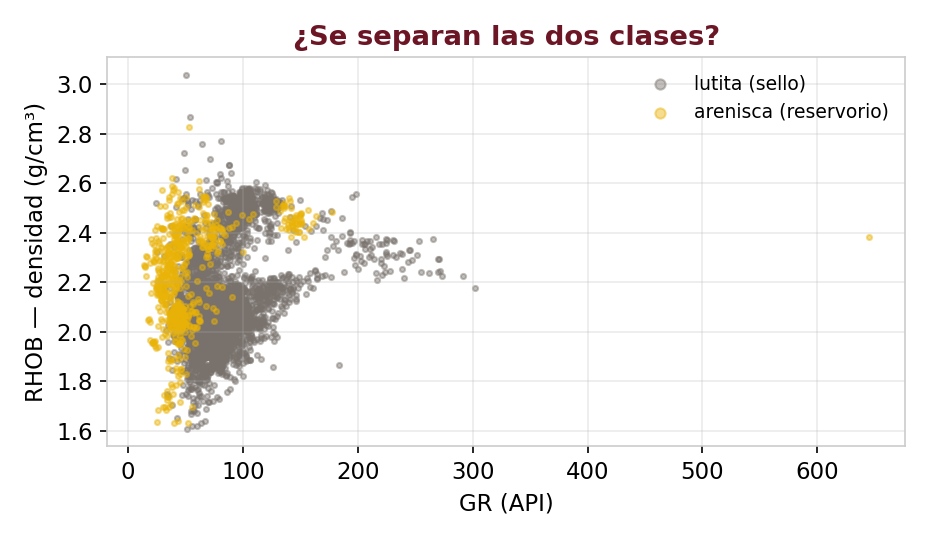
\includegraphics[width=\textwidth]{fig_clases.png}
    \end{column}
    \begin{column}{0.44\textwidth}
      {\footnotesize\color{textMuted}
      \begin{itemize}\setlength{\itemsep}{6pt}
        \item[{\color{codeGreen}\scriptsize\faCheck}]
          Buenas noticias: los colores \textbf{ocupan zonas distintas}.
          La arenisca vive a GR bajo.
        \item[{\color{arcaRed}\scriptsize\faExclamationTriangle}]
          Malas noticias: \textbf{se traslapan} en el medio.
          No hay una línea que separe perfecto.
        \item[{\color{arcaRed}\scriptsize\faArrowRight}]
          Por eso el modelo no dará certezas: dará
          \textbf{probabilidades}.
      \end{itemize}
      }
    \end{column}
  \end{columns}
\end{frame}

% ── EXPLORAR: DESBALANCE ─────────────────────────────────────────────────────
\begin{frame}[fragile,shrink=12]{Una Alerta Temprana: el Desbalance}
  \vspace{-4pt}
  {\small\color{arcaDark}\bfseries
    ¿Cuántos ejemplos hay de cada clase? La respuesta cambia todo lo que viene después.}

  \vspace{4pt}
  \begin{columns}[T]
    \begin{column}{0.50\textwidth}
      \begin{pyblock}
lito["LITH"].value_counts()
      \end{pyblock}
      \vspace{2pt}
      \begin{outputblock}
Shale        52011
Sandstone    10781
      \end{outputblock}
      \vspace{4pt}
      {\scriptsize\color{textMuted}
        \textbf{83\,\%} lutita, \textbf{17\,\%} arenisca.
        En geología es lo normal: la mayor parte de
        una columna sedimentaria es arcilla.}
    \end{column}
    \begin{column}{0.46\textwidth}
      \begin{tcolorbox}[colback=arcaGray, colframe=codeOrange, boxrule=0pt, leftrule=3pt,
        arc=3pt, left=6pt, right=6pt, top=5pt, bottom=5pt]
        {\scriptsize\color{codeOrange}\bfseries\faExclamationTriangle\hspace{4pt}Guarden este número}\\[4pt]
        {\scriptsize\color{textMuted}
          Un ``modelo'' que responda \textbf{siempre ``lutita''},
          sin mirar ningún dato, acertaría el
          \textbf{83\,\%} de las veces.\\[4pt]
          Volveremos a esto cuando hablemos de métricas.}
      \end{tcolorbox}
    \end{column}
  \end{columns}
\end{frame}

% ═════════════════════════════════════════════════════════════════════════════
\sectionframe{De la Recta a la Probabilidad}{Regresión logística}
% ═════════════════════════════════════════════════════════════════════════════

% ── POR QUÉ NO UNA RECTA ─────────────────────────────────────────────────────
\begin{frame}{¿Por Qué No Usar la Recta de la Clase Pasada?}
  \vspace{-6pt}
  {\small\color{arcaDark}\bfseries
    Podríamos poner \texttt{0} = lutita y \texttt{1} = arenisca, y ajustar una recta. Veamos qué pasa.}

  \vspace{4pt}
  \begin{columns}[T]
    \begin{column}{0.54\textwidth}
      \centering
      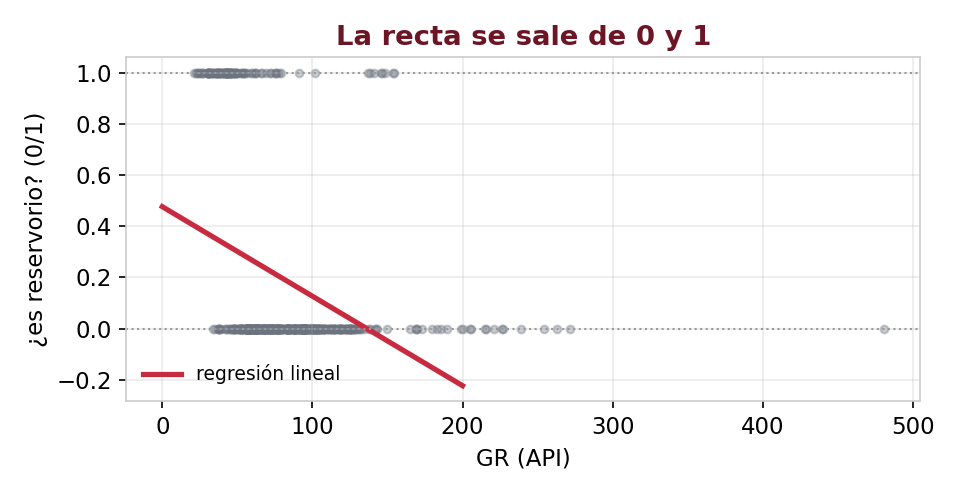
\includegraphics[width=\textwidth]{fig_recta_falla.png}
    \end{column}
    \begin{column}{0.42\textwidth}
      {\footnotesize\color{textMuted}
      \begin{itemize}\setlength{\itemsep}{6pt}
        \item[{\color{arcaRed}\scriptsize\faTimes}]
          La recta \textbf{no se detiene} en 0 ni en 1: predice
          \texttt{1.3} o \texttt{-0.2}.
        \item[{\color{arcaRed}\scriptsize\faQuestion}]
          ¿Qué significa ``1.3 de arenisca''? Nada.
        \item[{\color{codeGreen}\scriptsize\faLightbulb}]
          Necesitamos algo que \textbf{siempre} caiga entre
          0 y 1, para leerlo como \textbf{probabilidad}.
      \end{itemize}
      }
    \end{column}
  \end{columns}
\end{frame}

% ── LA SIGMOIDE ──────────────────────────────────────────────────────────────
\begin{frame}{La Solución: la Curva Sigmoide}
  \vspace{-6pt}
  {\small\color{arcaDark}\bfseries
    Una función que toma cualquier número y lo aplasta entre 0 y 1.}

  \vspace{4pt}
  \begin{columns}[T]
    \begin{column}{0.54\textwidth}
      \centering
      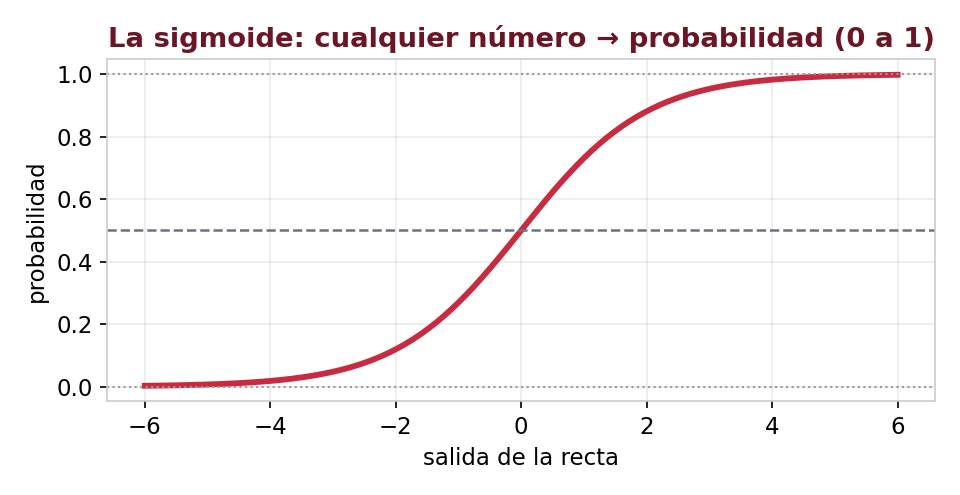
\includegraphics[width=\textwidth]{fig_sigmoide.png}
    \end{column}
    \begin{column}{0.42\textwidth}
      {\footnotesize\color{textMuted}
      \begin{itemize}\setlength{\itemsep}{5pt}
        \item[{\color{arcaRed}\scriptsize\faArrowRight}]
          Números muy negativos \(\to\) probabilidad
          cercana a \textbf{0}.
        \item[{\color{arcaRed}\scriptsize\faArrowRight}]
          Números muy positivos \(\to\) cercana a \textbf{1}.
        \item[{\color{arcaRed}\scriptsize\faArrowRight}]
          En el medio, una transición \textbf{suave}: ahí viven
          los casos dudosos.
      \end{itemize}
      }
      \vspace{4pt}
      {\scriptsize\color{arcaDark}\itshape
        \textbf{Regresión logística} = la misma recta de siempre,
        pasada por esta curva.}
    \end{column}
  \end{columns}
\end{frame}

% ── EN SKLEARN ───────────────────────────────────────────────────────────────
\begin{frame}[fragile,shrink=26]{Entrenar el Modelo: el Mismo Patrón de sklearn}
  \vspace{-4pt}
  {\small\color{arcaDark}\bfseries
    Cambia el modelo, \textbf{no el flujo}. Es el mismo \texttt{fit} de la clase pasada.}

  \vspace{4pt}
  \begin{columns}[T]
    \begin{column}{0.56\textwidth}
      \begin{pyblock}
from sklearn.linear_model import LogisticRegression

X = lito[["GR","RHOB","NPHI","DTC","RDEP"]]
y = lito["es_reservorio"]   # 1 = arenisca

X_tr, X_te, y_tr, y_te = train_test_split(
    X, y, test_size=0.25, random_state=42)

modelo = LogisticRegression(max_iter=1000)
modelo.fit(X_tr, y_tr)
      \end{pyblock}
    \end{column}
    \begin{column}{0.40\textwidth}
      {\scriptsize\color{textMuted}
      \begin{itemize}\setlength{\itemsep}{4pt}
        \item[{\color{arcaRed}\scriptsize\faArrowRight}]
          El target debe ser \textbf{0/1}, no texto.
        \item[{\color{arcaRed}\scriptsize\faArrowRight}]
          Igual que antes: \textbf{estandarizar} las features
          ayuda (escalas muy distintas).
        \item[{\color{codeGreen}\scriptsize\faCheck}]
          \texttt{.fit()}, \texttt{.predict()}, \texttt{.score()}:
          \textbf{idéntico} a la regresión lineal.
      \end{itemize}
      }
    \end{column}
  \end{columns}
\end{frame}

% ── QUÉ ES LA REGRESIÓN LOGÍSTICA ────────────────────────────────────────────
\begin{frame}{¿Qué es la Regresión Logística?}
  \vspace{-6pt}
  {\small\color{arcaDark}\bfseries
    Pese al nombre, \textbf{no} sirve para predecir números: es el modelo base para \textbf{clasificar}.}

  \vspace{6pt}
  \centering
  \begin{tikzpicture}[
    bx/.style={rectangle, rounded corners=5pt, minimum height=1.05cm,
      minimum width=3.05cm, align=center, font=\scriptsize, text=white},
    ar/.style={-{Stealth[length=6pt]}, line width=1.3pt, arcaRed},
    node distance=0.62cm]
    \node[bx, fill=arcaDark] (a) {\faSlidersH\\[2pt]\textbf{Registros}\\{\tiny GR, RHOB, NPHI\ldots}};
    \node[bx, fill=arcaRed, right=of a] (b) {\faCalculator\\[2pt]\textbf{Una recta}\\{\tiny suma ponderada}};
    \node[bx, fill=udlaCrimson, right=of b] (c) {\faWaveSquare\\[2pt]\textbf{Sigmoide}\\{\tiny aplasta a 0--1}};
    \node[bx, fill=arcaDark!85, right=of c] (d) {\faPercent\\[2pt]\textbf{Probabilidad}\\{\tiny p.ej. 0.78}};
    \node[bx, fill=codeGreen!85!black, right=of d] (e) {\faTags\\[2pt]\textbf{Etiqueta}\\{\tiny según el umbral}};
    \draw[ar] (a)--(b); \draw[ar] (b)--(c); \draw[ar] (c)--(d); \draw[ar] (d)--(e);
  \end{tikzpicture}

  \vspace{8pt}
  {\footnotesize\color{textMuted}
  \begin{itemize}\setlength{\itemsep}{4pt}
    \item[{\color{arcaRed}\scriptsize\faArrowRight}]
      Por dentro es \textbf{la misma recta} de la clase pasada: cada registro
      aporta con su peso (\(m_1\texttt{GR} + m_2\texttt{RHOB} + \ldots\)).
    \item[{\color{arcaRed}\scriptsize\faArrowRight}]
      La diferencia: el resultado \textbf{pasa por la sigmoide}, que lo convierte
      en una \textbf{probabilidad}.
    \item[{\color{codeGreen}\scriptsize\faCheck}]
      Se llama ``regresión'' porque \textbf{internamente} hace una regresión;
      lo que \textbf{entrega} es una clasificación.
  \end{itemize}
  }
\end{frame}

% ── PARA QUÉ SE USA ──────────────────────────────────────────────────────────
\begin{frame}[shrink=8]{¿Para Qué se Usa? ¿Por Qué Empezar por Ella?}
  \vspace{-4pt}
  {\small\color{arcaDark}\bfseries
    Es el \textbf{primer modelo} que se prueba en cualquier problema de clasificación --- y muchas veces el que queda.}

  \vspace{6pt}
  \begin{columns}[T]
    \begin{column}{0.48\textwidth}
      {\footnotesize\color{arcaDark}\bfseries\faCheck\hspace{4pt}Sus fortalezas:}
      \vspace{3pt}
      {\scriptsize\color{textMuted}
      \begin{itemize}\setlength{\itemsep}{4pt}
        \item[{\color{codeGreen}\scriptsize\faEye}]
          \textbf{Se puede explicar}: cada coeficiente dice cómo influye
          cada registro. Auditable ante un cliente o un regulador.
        \item[{\color{codeGreen}\scriptsize\faBolt}]
          \textbf{Rápida} y estable, incluso con pocos datos.
        \item[{\color{codeGreen}\scriptsize\faRuler}]
          Sirve de \textbf{línea base}: si un modelo complejo no la supera,
          no vale la pena su complejidad.
      \end{itemize}
      }
    \end{column}
    \begin{column}{0.48\textwidth}
      {\footnotesize\color{arcaDark}\bfseries\faTimes\hspace{4pt}Sus límites:}
      \vspace{3pt}
      {\scriptsize\color{textMuted}
      \begin{itemize}\setlength{\itemsep}{4pt}
        \item[{\color{arcaRed}\scriptsize\faExclamationTriangle}]
          Separa las clases con una \textbf{frontera recta}. Si la frontera
          real es curva, se queda corta.
        \item[{\color{arcaRed}\scriptsize\faExclamationTriangle}]
          Le afectan los \textbf{outliers} y las escalas muy distintas
          (por eso estandarizamos).
      \end{itemize}
      }
      \vspace{4pt}
      {\scriptsize\color{arcaDark}\itshape
        Para fronteras curvas: árboles y bosques
        --- las próximas clases.}
    \end{column}
  \end{columns}

  \vspace{5pt}
  \centering
  {\scriptsize\color{textMuted}
    Usos típicos en la industria: litología \(\cdot\) ¿pozo productor o seco? \(\cdot\)
    ¿fallará el equipo? \(\cdot\) ¿hay riesgo de pega de tubería?}
\end{frame}

% ── INTERPRETAR COEFICIENTES ─────────────────────────────────────────────────
\begin{frame}[fragile,shrink=22]{Leer el Modelo: ¿Qué Aprendió?}
  \vspace{-4pt}
  {\small\color{arcaDark}\bfseries
    Su gran ventaja: podemos \textbf{abrirlo} y ver en qué se fijó (con las features estandarizadas).}

  \vspace{4pt}
  \begin{columns}[T]
    \begin{column}{0.50\textwidth}
      \begin{pyblock}
pd.Series(modelo.coef_[0],
          index=X.columns).round(2)
      \end{pyblock}
      \vspace{2pt}
      \begin{outputblock}
NPHI    -3.36
RHOB    -2.59
GR      -1.65
DTC     -0.84
RDEP     0.01
      \end{outputblock}
    \end{column}
    \begin{column}{0.46\textwidth}
      {\scriptsize\color{textMuted}
      \begin{itemize}\setlength{\itemsep}{4pt}
        \item[{\color{arcaRed}\scriptsize\faArrowRight}]
          Coeficiente \textbf{negativo} = ese registro alto
          \textbf{empuja hacia lutita}.
        \item[{\color{codeGreen}\scriptsize\faCheck}]
          \texttt{GR} negativo: mucha radioactividad
          \(\to\) arcilla. \textbf{Coincide con la geología.}
        \item[{\color{codeGreen}\scriptsize\faCheck}]
          \texttt{NPHI} y \texttt{RHOB} son los que más pesan.
        \item[{\color{arcaRed}\scriptsize\faTimes}]
          \texttt{RDEP} \(\approx 0\): no aporta a distinguir
          la litología.
      \end{itemize}
      }
    \end{column}
  \end{columns}

  \vspace{3pt}
  {\scriptsize\color{arcaDark}
    \faLightbulb[regular]\hspace{3pt}%
    Que el modelo ``piense'' como la física \textbf{es una señal de que no está memorizando ruido}.}
\end{frame}

% ── PROBABILIDAD Y UMBRAL ────────────────────────────────────────────────────
\begin{frame}[fragile,shrink=20]{Lo Que Realmente Devuelve: Probabilidades}
  \vspace{-4pt}
  {\small\color{arcaDark}\bfseries
    El modelo no dice ``arenisca''. Dice ``\textbf{78\,\% de probabilidad} de arenisca''.}

  \vspace{4pt}
  \begin{columns}[T]
    \begin{column}{0.54\textwidth}
      \begin{pyblock}
proba = modelo.predict_proba(X_te)[:, 1]
proba[:4].round(2)
      \end{pyblock}
      \vspace{2pt}
      \begin{outputblock}[]
[0.03  0.78  0.41  0.95]
      \end{outputblock}
      \vspace{3pt}
      \begin{pyblock}
pred = (proba >= 0.5).astype(int)
      \end{pyblock}
    \end{column}
    \begin{column}{0.42\textwidth}
      {\scriptsize\color{textMuted}
      \begin{itemize}\setlength{\itemsep}{4pt}
        \item[{\color{arcaRed}\scriptsize\faArrowRight}]
          Para dar una respuesta hay que fijar un
          \textbf{umbral}: por defecto \textbf{0.5}.
        \item[{\color{arcaRed}\scriptsize\faExclamationTriangle}]
          Ese 0.5 es una \textbf{convención}, no una ley.
        \item[{\color{codeGreen}\scriptsize\faStar}]
          \textbf{Moverlo es la decisión más importante
          de la clase.} Lo haremos al final.
      \end{itemize}
      }
    \end{column}
  \end{columns}
\end{frame}

% ═════════════════════════════════════════════════════════════════════════════
\sectionframe{Las Métricas}{Aquí se decide si el modelo sirve}
% ═════════════════════════════════════════════════════════════════════════════

% ── ANALOGÍA DEL DETECTOR DE GAS ─────────────────────────────────────────────
\begin{frame}[shrink=8]{Antes de las Fórmulas: el Detector de Gas}
  \vspace{-4pt}
  {\small\color{arcaDark}\bfseries
    Ustedes ya saben evaluar un clasificador: conviven con uno todos los días.}

  \vspace{6pt}
  \begin{columns}[T]
    \begin{column}{0.48\textwidth}
      \begin{tcolorbox}[colback=arcaGray, colframe=arcaRed, boxrule=0pt, leftrule=3pt,
        arc=3pt, left=6pt, right=6pt, top=5pt, bottom=5pt]
        {\scriptsize\color{arcaRed}\bfseries Detector que NUNCA suena}\\[4pt]
        {\scriptsize\color{textMuted}
          Como casi nunca hay fuga, acierta el
          \textbf{99.9\,\%} de los días.\\[4pt]
          \textbf{Accuracy altísima\ldots{} y es un adorno:}
          el día de la fuga no avisa.}
      \end{tcolorbox}
    \end{column}
    \begin{column}{0.48\textwidth}
      \begin{tcolorbox}[colback=arcaGray, colframe=codeOrange, boxrule=0pt, leftrule=3pt,
        arc=3pt, left=6pt, right=6pt, top=5pt, bottom=5pt]
        {\scriptsize\color{codeOrange}\bfseries Detector que suena SIEMPRE}\\[4pt]
        {\scriptsize\color{textMuted}
          No se le escapa ninguna fuga jamás.\\[4pt]
          \textbf{Pero nadie le cree:} tantas falsas
          alarmas que la cuadrilla lo ignora.}
      \end{tcolorbox}
    \end{column}
  \end{columns}

  \vspace{8pt}
  {\footnotesize\color{textMuted}
  \begin{itemize}\setlength{\itemsep}{4pt}
    \item[{\color{arcaRed}\scriptsize\faArrowRight}]
      Nadie evalúa un detector de gas por su \textbf{\% de aciertos}. Se evalúa por
      \textbf{cuántas fugas detecta} y \textbf{cuántas veces molesta en falso}.
    \item[{\color{codeGreen}\scriptsize\faCheck}]
      Esas dos preguntas tienen nombre técnico: \textbf{recall} y \textbf{precision}.
      Ya las entienden --- ahora les ponemos el nombre.
  \end{itemize}
  }
\end{frame}

% ── ACCURACY ENGAÑA ──────────────────────────────────────────────────────────
\begin{frame}[fragile,shrink=15]{Accuracy: la Métrica que Engaña}
  \vspace{-4pt}
  {\small\color{arcaDark}\bfseries
    \textbf{Accuracy} = \% de aciertos. Es la primera que todos miran\ldots y la más peligrosa.}

  \vspace{4pt}
  \begin{columns}[T]
    \begin{column}{0.48\textwidth}
      \begin{pyblock}
modelo.score(X_te, y_te)
      \end{pyblock}
      \vspace{2pt}
      \begin{outputblock}[]
0.944
      \end{outputblock}
      \vspace{4pt}
      {\scriptsize\color{textMuted}
        94.4\,\% de aciertos. \textbf{Excelente}, ¿no?}
    \end{column}
    \begin{column}{0.48\textwidth}
      \begin{tcolorbox}[colback=arcaGray, colframe=arcaRed, boxrule=0pt, leftrule=3pt,
        arc=3pt, left=6pt, right=6pt, top=5pt, bottom=5pt]
        {\scriptsize\color{arcaRed}\bfseries\faExclamationTriangle\hspace{4pt}Recuerden el desbalance}\\[4pt]
        {\scriptsize\color{textMuted}
          Responder \textbf{siempre ``lutita''}, sin mirar
          nada, da \textbf{82.8\,\%}.\\[4pt]
          Nuestro modelo ``excelente'' solo mejora
          \textbf{12 puntos} sobre no pensar.}
      \end{tcolorbox}
    \end{column}
  \end{columns}

  \vspace{5pt}
  {\footnotesize\color{arcaDark}
    \faLightbulb[regular]\hspace{4pt}%
    Con clases desbalanceadas, la accuracy \textbf{esconde} lo que de verdad importa:
    ¿encontramos las zonas de reservorio, que son las escasas?}
\end{frame}

% ── MATRIZ DE CONFUSIÓN ──────────────────────────────────────────────────────
\begin{frame}{Abrir la Caja: la Matriz de Confusión}
  \vspace{-6pt}
  {\small\color{arcaDark}\bfseries
    En vez de un número, los \textbf{cuatro} resultados posibles --- con nombre de negocio.}

  \vspace{2pt}
  \begin{columns}[T]
    \begin{column}{0.52\textwidth}
      \centering
      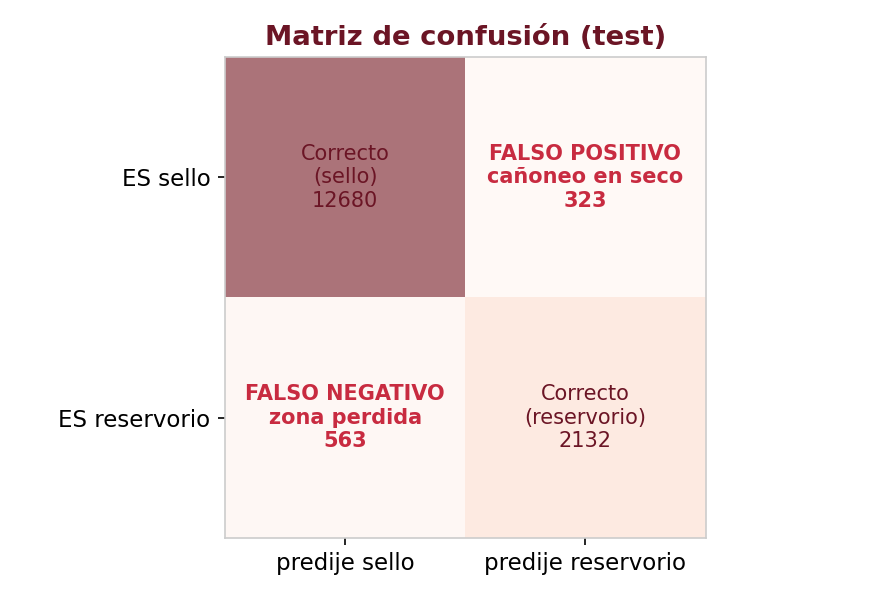
\includegraphics[width=\textwidth]{fig_confusion.png}
    \end{column}
    \begin{column}{0.44\textwidth}
      {\scriptsize\color{textMuted}
      \begin{itemize}\setlength{\itemsep}{5pt}
        \item[{\color{codeGreen}\scriptsize\faCheck}]
          \textbf{Aciertos} (diagonal): 12\,680 sellos y
          2\,132 reservorios bien identificados.
        \item[{\color{arcaRed}\scriptsize\faTimes}]
          \textbf{323 falsos positivos}: dijimos reservorio
          y era sello \(\to\) \textit{cañoneo en seco}.
        \item[{\color{arcaRed}\scriptsize\faTimes}]
          \textbf{563 falsos negativos}: dijimos sello
          y era reservorio \(\to\) \textit{zona productiva perdida}.
      \end{itemize}
      }
      \vspace{3pt}
      {\scriptsize\color{arcaDark}\itshape
        La accuracy sumaba todo esto en un solo número
        y \textbf{escondía} los 563.}
    \end{column}
  \end{columns}
\end{frame}

% ── PRECISION Y RECALL ───────────────────────────────────────────────────────
\begin{frame}[shrink=8]{Las Dos Preguntas: Precision y Recall}
  \vspace{-4pt}
  {\small\color{arcaDark}\bfseries
    Dos métricas que responden preguntas \textbf{distintas} sobre la misma matriz.}

  \vspace{6pt}
  \begin{columns}[T]
    \begin{column}{0.48\textwidth}
      \begin{tcolorbox}[colback=arcaGray, colframe=codeBlue, boxrule=0pt, leftrule=3pt,
        arc=3pt, left=6pt, right=6pt, top=5pt, bottom=5pt]
        {\footnotesize\color{codeBlue}\bfseries PRECISION = 0.87}\\[4pt]
        {\scriptsize\color{arcaDark}\itshape
          ``De todas las veces que dije \textbf{reservorio},
          ¿cuántas acerté?''}\\[5pt]
        {\scriptsize\color{textMuted}
          Mide si podemos \textbf{confiar} cuando el modelo dice que sí.\\[4pt]
          \textbf{Importa cuando actuar en falso es caro}
          (cañonear en seco).}
      \end{tcolorbox}
    \end{column}
    \begin{column}{0.48\textwidth}
      \begin{tcolorbox}[colback=arcaGray, colframe=arcaRed, boxrule=0pt, leftrule=3pt,
        arc=3pt, left=6pt, right=6pt, top=5pt, bottom=5pt]
        {\footnotesize\color{arcaRed}\bfseries RECALL = 0.79}\\[4pt]
        {\scriptsize\color{arcaDark}\itshape
          ``De todas las zonas que \textbf{eran} reservorio,
          ¿cuántas encontré?''}\\[5pt]
        {\scriptsize\color{textMuted}
          Mide cuánto se nos \textbf{escapa}.\\[4pt]
          \textbf{Importa cuando perderse algo es caro}
          (dejar petróleo en el subsuelo).}
      \end{tcolorbox}
    \end{column}
  \end{columns}

  \vspace{8pt}
  \centering
  {\footnotesize\color{arcaDark}
    Nuestro recall de \textbf{0.79} significa: de cada 10 zonas de reservorio,
    \textbf{se nos escapan 2}.}
\end{frame}

% ── DE DÓNDE SALE CADA MÉTRICA ───────────────────────────────────────────────
\begin{frame}{De Dónde Sale Cada Métrica}
  \vspace{-6pt}
  {\small\color{arcaDark}\bfseries
    Ambas salen de la misma matriz. La diferencia es \textbf{qué se toma como referencia}.}

  \vspace{6pt}
  \centering
  \begin{tikzpicture}[font=\scriptsize, cell/.style={rectangle, draw=arcaLightGray,
      minimum width=2.6cm, minimum height=1.05cm, align=center}]
    % --- RECALL: fila de "ES reservorio" ---
    \begin{scope}[xshift=-3.9cm]
      \node[font=\scriptsize\bfseries, text=arcaRed] at (0,1.5) {RECALL = de las que ERAN};
      \node[cell, fill=white] (a1) at (-1.35,0.55) {563};
      \node[cell, fill=white] (a2) at ( 1.35,0.55) {2\,132};
      \node[cell, fill=arcaRed!22] (a3) at (-1.35,-0.55) {\textbf{563}};
      \node[cell, fill=arcaRed!22] (a4) at ( 1.35,-0.55) {\textbf{2\,132}};
      \node[font=\tiny, text=textMuted, anchor=east] at (-2.75,0.55) {ES sello};
      \node[font=\tiny\bfseries, text=arcaRed, anchor=east] at (-2.75,-0.55) {ES reservorio};
      \node[font=\tiny, text=arcaRed] at (0,-1.35) {mira la FILA: 2132/(2132+563) = \textbf{0.79}};
    \end{scope}
    % --- PRECISION: columna de "predije reservorio" ---
    \begin{scope}[xshift=3.9cm]
      \node[font=\scriptsize\bfseries, text=codeBlue] at (0,1.5) {PRECISION = de las que DIJE};
      \node[cell, fill=white] (b1) at (-1.35,0.55) {12\,680};
      \node[cell, fill=codeBlue!18] (b2) at ( 1.35,0.55) {\textbf{323}};
      \node[cell, fill=white] (b3) at (-1.35,-0.55) {563};
      \node[cell, fill=codeBlue!18] (b4) at ( 1.35,-0.55) {\textbf{2\,132}};
      \node[font=\tiny, text=textMuted] at (-1.35,-1.28) {predije sello};
      \node[font=\tiny\bfseries, text=codeBlue] at (1.35,-1.28) {predije reservorio};
      \node[font=\tiny, text=codeBlue] at (0,-1.75) {mira la COLUMNA: 2132/(2132+323) = \textbf{0.87}};
    \end{scope}
  \end{tikzpicture}

  \vspace{8pt}
  {\footnotesize\color{textMuted}
    \faLightbulb[regular]\hspace{4pt}%
    Truco para no confundirlas: \textbf{recall} mira la \textbf{realidad}
    (¿cuánto de lo que existía encontré?); \textbf{precision} mira \textbf{mis anuncios}
    (¿cuánto de lo que dije era cierto?).}
\end{frame}

% ── CUÁL PRIORIZAR ───────────────────────────────────────────────────────────
\begin{frame}[shrink=8]{¿Cuál Priorizar? Depende del Daño}
  \vspace{-4pt}
  {\small\color{arcaDark}\bfseries
    No hay una mejor: hay una que importa \textbf{más en su problema}.}

  \vspace{5pt}
  \centering
  {\scriptsize
  \renewcommand{\arraystretch}{1.45}
  \begin{tabular}{@{}p{4.6cm} p{2.4cm} p{4.4cm}@{}}
    \toprule
    {\bfseries\color{arcaDark} Situación} & {\bfseries\color{arcaRed} Priorizar}
      & {\bfseries\color{arcaDark} Por qué} \\
    \midrule
    \rowcolor{arcaGray}
    Detectar zonas de reservorio & \textbf{Recall}
      & perderse una zona productiva cuesta reservas para siempre \\
    Alarma de fuga de gas & \textbf{Recall}
      & no detectar una fuga es un evento de seguridad \\
    \rowcolor{arcaGray}
    Recomendar un workover de \$2M & \textbf{Precision}
      & si nos equivocamos gastamos el presupuesto en vano \\
    Parar la producción por alerta & \textbf{Precision}
      & cada parada en falso cuesta producción diferida \\
    \bottomrule
  \end{tabular}
  }

  \vspace{7pt}
  {\footnotesize\color{textMuted}
  \begin{itemize}\setlength{\itemsep}{3pt}
    \item[{\color{arcaRed}\scriptsize\faExclamationTriangle}]
      Subir una \textbf{casi siempre} baja la otra. No se puede maximizar ambas.
    \item[{\color{codeGreen}\scriptsize\faCheck}]
      La pregunta correcta no es ``¿cuál es mejor?'' sino
      \textbf{``¿cuál error hace más daño aquí?''}
  \end{itemize}
  }
\end{frame}

% ── F1 Y CÓDIGO ──────────────────────────────────────────────────────────────
\begin{frame}[fragile,shrink=25]{F1 y las Métricas en Código}
  \vspace{-4pt}
  {\small\color{arcaDark}\bfseries
    \texttt{F1} combina precision y recall en un solo número (útil para comparar modelos).}

  \vspace{4pt}
  \begin{columns}[T]
    \begin{column}{0.56\textwidth}
      \begin{pyblock}
from sklearn.metrics import (accuracy_score,
    precision_score, recall_score, f1_score,
    confusion_matrix)

pred = modelo.predict(X_te)

print(accuracy_score(y_te, pred))
print(precision_score(y_te, pred))
print(recall_score(y_te, pred))
print(f1_score(y_te, pred))
      \end{pyblock}
    \end{column}
    \begin{column}{0.40\textwidth}
      \begin{outputblock}[]
0.944   accuracy
0.868   precision
0.791   recall
0.828   f1
      \end{outputblock}
      \vspace{4pt}
      {\scriptsize\color{textMuted}
        \textbf{F1} castiga los desequilibrios: si el recall
        es bajo, el F1 baja aunque la precision
        sea alta.}
    \end{column}
  \end{columns}
\end{frame}

% ── CRITERIOS ────────────────────────────────────────────────────────────────
\begin{frame}[shrink=12]{¿Cuál Métrica Uso? Criterios y Valores}
  \vspace{-4pt}
  \centering
  {\scriptsize
  \renewcommand{\arraystretch}{1.45}
  \begin{tabular}{@{}l p{4.3cm} p{4.7cm}@{}}
    \toprule
    {\bfseries\color{arcaRed} Métrica} & {\bfseries\color{arcaDark} Cuándo elegirla}
      & {\bfseries\color{arcaDark} Qué es ``aceptable''} \\
    \midrule
    \rowcolor{arcaGray}
    Accuracy & solo si las clases están \textbf{balanceadas}
      & debe superar \textbf{claramente} el \% de la clase mayoritaria \\
    Precision & cuando una \textbf{falsa alarma} cuesta cara
      & \(>0.8\) en decisiones operativas \\
    \rowcolor{arcaGray}
    Recall & cuando \textbf{perderse un caso} cuesta caro
      & \(>0.9\) si el caso perdido es crítico (seguridad, reservas) \\
    F1 & comparar modelos con clases desbalanceadas
      & \(>0.7\) razonable \(\cdot\) \(>0.85\) muy bueno \\
    \bottomrule
  \end{tabular}
  }

  \vspace{8pt}
  {\footnotesize\color{textMuted}
  \begin{itemize}\setlength{\itemsep}{3pt}
    \item[{\color{arcaRed}\scriptsize\faExclamationTriangle}]
      \textbf{Nunca} reportar una sola métrica. Precision y recall
      \textbf{siempre} van juntas.
    \item[{\color{arcaRed}\scriptsize\faArrowRight}]
      Y todas, \textbf{sobre el test}.
  \end{itemize}
  }
\end{frame}

% ═════════════════════════════════════════════════════════════════════════════
\sectionframe{El Costo de Negocio}{Lo que separa a un ingeniero de un operador de librerías}
% ═════════════════════════════════════════════════════════════════════════════

% ── LOS ERRORES NO CUESTAN IGUAL ─────────────────────────────────────────────
\begin{frame}{Los Dos Errores NO Cuestan lo Mismo}
  \vspace{-6pt}
  {\small\color{arcaDark}\bfseries
    Hasta ahora contamos errores. Ahora vamos a \textbf{ponerles precio}.}

  \vspace{8pt}
  \begin{columns}[T]
    \begin{column}{0.48\textwidth}
      \begin{tcolorbox}[colback=arcaGray, colframe=codeOrange, boxrule=0pt, leftrule=3pt,
        arc=3pt, left=6pt, right=6pt, top=5pt, bottom=5pt]
        {\scriptsize\color{codeOrange}\bfseries FALSO POSITIVO}\\[3pt]
        {\scriptsize\color{arcaDark}\itshape ``dije reservorio, era sello''}\\[5pt]
        {\scriptsize\color{textMuted}
          Cañoneamos y completamos un intervalo que
          no produce.\\[4pt]
          \textbf{Costo:} el trabajo de completación
          desperdiciado. Es \textbf{dinero gastado}, medible,
          y se detecta rápido.}
      \end{tcolorbox}
    \end{column}
    \begin{column}{0.48\textwidth}
      \begin{tcolorbox}[colback=arcaGray, colframe=arcaRed, boxrule=0pt, leftrule=3pt,
        arc=3pt, left=6pt, right=6pt, top=5pt, bottom=5pt]
        {\scriptsize\color{arcaRed}\bfseries FALSO NEGATIVO}\\[3pt]
        {\scriptsize\color{arcaDark}\itshape ``dije sello, era reservorio''}\\[5pt]
        {\scriptsize\color{textMuted}
          Nunca completamos esa zona.\\[4pt]
          \textbf{Costo:} las reservas que esa zona habría
          producido \textbf{durante toda la vida del pozo}.
          Y \textbf{nadie se entera}: no aparece en ningún reporte.}
      \end{tcolorbox}
    \end{column}
  \end{columns}

  \vspace{8pt}
  \centering
  {\footnotesize\color{arcaDark}
    En este problema, \textbf{perder una zona productiva} suele costar
    \textbf{mucho más} que un cañoneo en seco.}
\end{frame}

% ── EL UMBRAL ────────────────────────────────────────────────────────────────
\begin{frame}{El Umbral: la Perilla que Casi Nadie Toca}
  \vspace{-6pt}
  {\small\color{arcaDark}\bfseries
    Bajar el umbral = ser \textbf{más generoso} al declarar reservorio. Encontramos más\ldots y nos equivocamos más.}

  \vspace{4pt}
  \begin{columns}[T]
    \begin{column}{0.54\textwidth}
      \centering
      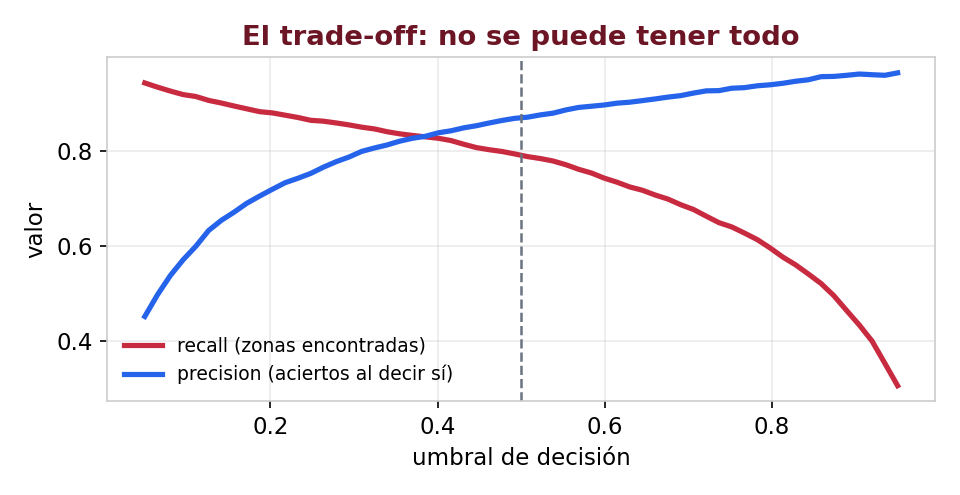
\includegraphics[width=\textwidth]{fig_umbral.png}
    \end{column}
    \begin{column}{0.42\textwidth}
      {\footnotesize\color{textMuted}
      \begin{itemize}\setlength{\itemsep}{5pt}
        \item[{\color{arcaRed}\scriptsize\faArrowDown}]
          Umbral \textbf{bajo}: recall sube (encuentro casi todo),
          precision baja (muchas falsas alarmas).
        \item[{\color{arcaRed}\scriptsize\faArrowUp}]
          Umbral \textbf{alto}: precision sube (cuando digo sí,
          acierto), pero se me escapan zonas.
        \item[{\color{codeGreen}\scriptsize\faStar}]
          \textbf{No existe el umbral ``correcto'' en abstracto.}
          Depende de qué error cuesta más.
      \end{itemize}
      }
    \end{column}
  \end{columns}
\end{frame}

% ── LA TABLA DE COSTO ────────────────────────────────────────────────────────
\begin{frame}[shrink=10]{Ponerle Precio: la Matriz de Costos}
  \vspace{-4pt}
  {\small\color{arcaDark}\bfseries
    Supongamos, con el equipo de yacimientos, que \textbf{perder una zona cuesta 10 veces} un cañoneo en seco.}

  \vspace{5pt}
  \centering
  {\footnotesize
  \renewcommand{\arraystretch}{1.4}
  \begin{tabular}{@{}c c c c@{}}
    \toprule
    {\bfseries\color{arcaRed} Umbral} & {\bfseries\color{arcaDark} Zonas perdidas (FN)}
      & {\bfseries\color{arcaDark} Cañoneos en seco (FP)}
      & {\bfseries\color{arcaDark} Costo total (FN\(\times\)10 + FP)} \\
    \midrule
    0.50 \tiny(por defecto) & 563 & 323 & 5\,953 \\
    \rowcolor{arcaGray}
    0.40 & 469 & 434 & 5\,124 \\
    0.30 & 400 & 603 & 4\,603 \\
    \rowcolor{arcaGray}
    0.25 & 368 & 760 & 4\,440 \\
    0.20 & 324 & 939 & {\color{codeGreen}\bfseries 4\,179} \\
    \bottomrule
  \end{tabular}
  }

  \vspace{8pt}
  {\footnotesize\color{textMuted}
    \faLightbulb[regular]\hspace{4pt}%
    Al bajar el umbral aceptamos \textbf{más} cañoneos en seco (323 \(\to\) 939)
    para rescatar \textbf{239 zonas productivas}. En dinero, el cambio
    \textbf{conviene}.}
\end{frame}

% ── LA CURVA DE COSTO ────────────────────────────────────────────────────────
\begin{frame}{El Umbral que Minimiza el Costo}
  \vspace{-6pt}
  {\small\color{arcaDark}\bfseries
    Si graficamos el costo total contra el umbral, aparece el punto óptimo.}

  \vspace{4pt}
  \begin{columns}[T]
    \begin{column}{0.56\textwidth}
      \centering
      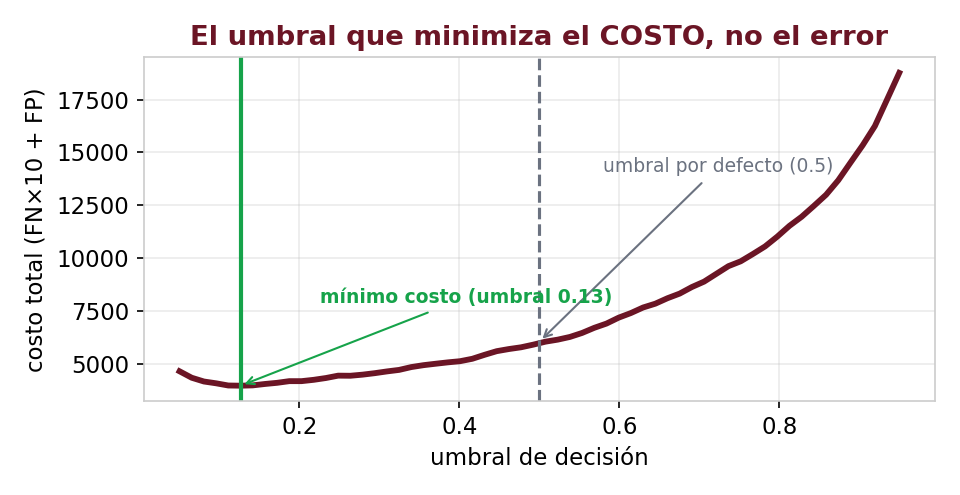
\includegraphics[width=\textwidth]{fig_costo.png}
    \end{column}
    \begin{column}{0.40\textwidth}
      {\footnotesize\color{textMuted}
      \begin{itemize}\setlength{\itemsep}{6pt}
        \item[{\color{arcaRed}\scriptsize\faArrowRight}]
          El umbral por defecto (\textbf{0.5}) cuesta \textbf{5\,953}.
        \item[{\color{codeGreen}\scriptsize\faCheck}]
          El umbral óptimo (\textbf{0.13}) cuesta \textbf{3\,962}.
        \item[{\color{codeGreen}\scriptsize\faTrophy}]
          \textbf{33\,\% menos costo} --- sin cambiar el modelo,
          sin más datos: solo \textbf{moviendo una perilla}.
      \end{itemize}
      }
    \end{column}
  \end{columns}
\end{frame}

% ── EL VEREDICTO ─────────────────────────────────────────────────────────────
\begin{frame}[shrink=12]{El Veredicto: Peor Modelo, Mejor Negocio}
  \vspace{-6pt}
  \centering
  {\footnotesize
  \renewcommand{\arraystretch}{1.5}
  \begin{tabular}{@{}l c c@{}}
    \toprule
     & {\bfseries\color{textMuted} Umbral 0.5 (por defecto)} & {\bfseries\color{codeGreen} Umbral 0.13 (por costo)} \\
    \midrule
    \rowcolor{arcaGray}
    Accuracy & \textbf{0.944} & 0.895 \\
    Recall & 0.791 & \textbf{0.905} \\
    Zonas perdidas & 563 & \textbf{257} \\
    \rowcolor{arcaGray}
    \textbf{Costo total} & 5\,953 & {\color{codeGreen}\bfseries 3\,962} \\
    \bottomrule
  \end{tabular}
  }

  \vspace{10pt}
  \begin{tcolorbox}[colback=arcaGray, colframe=arcaRed, boxrule=0pt, leftrule=3pt,
    arc=3pt, left=8pt, right=8pt, top=6pt, bottom=6pt, width=0.88\textwidth]
    {\footnotesize\color{arcaDark}
      El segundo modelo tiene \textbf{peor accuracy}. Un reporte automático
      diría que es \textbf{inferior}.\\[4pt]
      Y sin embargo es el que \textbf{le conviene a la empresa}.}
  \end{tcolorbox}

  \vspace{8pt}
  {\footnotesize\color{arcaDark}
    \faStar\hspace{4pt}%
    \textbf{Eso es lo que separa} al ingeniero que entiende el negocio
    del que solo corre \texttt{.fit()} y reporta la accuracy.}
\end{frame}

% ── CÓMO SE HACE EN LA PRÁCTICA ──────────────────────────────────────────────
\begin{frame}[shrink=8]{Cómo se Hace Esto en la Práctica}
  \vspace{-4pt}
  {\small\color{arcaDark}\bfseries
    El paso que ningún curso de ML enseña y todo proyecto real necesita.}

  \vspace{8pt}
  {\footnotesize\color{textMuted}
  \begin{enumerate}\setlength{\itemsep}{7pt}
    \item[{\color{arcaRed}\bfseries 1.}]
      \textbf{Preguntar, no asumir.} Sentarse con yacimientos, producción o
      finanzas: \textit{¿cuánto cuesta cada error?} Casi nunca está escrito.
    \item[{\color{arcaRed}\bfseries 2.}]
      \textbf{Basta la proporción.} No hace falta el número exacto:
      con saber que un error cuesta \(\sim\)10 veces el otro, ya se puede decidir.
    \item[{\color{arcaRed}\bfseries 3.}]
      \textbf{Elegir el umbral con esa proporción}, no con el 0.5 de fábrica.
    \item[{\color{arcaRed}\bfseries 4.}]
      \textbf{Reportar en el lenguaje del que decide:}
      no ``recall 0.91'' sino \textit{``recuperamos 306 zonas que antes
      se perdían, a cambio de 1\,069 cañoneos adicionales''}.
  \end{enumerate}
  }
\end{frame}

% ═════════════════════════════════════════════════════════════════════════════
\sectionframe{Cierre}{Lo que se llevan hoy}
% ═════════════════════════════════════════════════════════════════════════════

% ── FLUJO ────────────────────────────────────────────────────────────────────
\begin{frame}{El Flujo de un Problema de Clasificación}
  \vspace{-4pt}
  \centering
  \begin{tikzpicture}[
    mlstep/.style={rectangle, rounded corners=5pt, fill=arcaGray, draw=arcaLightGray,
      minimum width=2.4cm, minimum height=1.15cm, align=center,
      font=\scriptsize, text=textDark},
    num/.style={circle, fill=arcaRed, text=white, font=\scriptsize\bfseries,
      minimum size=0.5cm, inner sep=0pt},
    ar/.style={-{Stealth[length=5pt]}, line width=1.2pt, arcaRed},
    node distance=0.5cm]
    \node[mlstep] (s1) {\faDatabase\\[2pt]Datos\\etiquetados};
    \node[mlstep, right=of s1] (s2) {\faCut\\[2pt]Train /\\Test};
    \node[mlstep, right=of s2] (s3) {\faRobot\\[2pt]Entrenar\\\texttt{.fit}};
    \node[mlstep, right=of s3] (s4) {\faTable\\[2pt]Matriz de\\confusión};
    \node[mlstep, right=of s4, fill=arcaRed!12, draw=arcaRed] (s5) {\faDollarSign\\[2pt]Umbral\\por costo};
    \node[num, above=0.1cm of s1] {1}; \node[num, above=0.1cm of s2] {2};
    \node[num, above=0.1cm of s3] {3}; \node[num, above=0.1cm of s4] {4};
    \node[num, above=0.1cm of s5] {5};
    \draw[ar] (s1)--(s2); \draw[ar] (s2)--(s3); \draw[ar] (s3)--(s4); \draw[ar] (s4)--(s5);
  \end{tikzpicture}

  \vspace{10pt}
  {\footnotesize\color{textMuted}
  \begin{itemize}\setlength{\itemsep}{4pt}
    \item[{\color{codeGreen}\scriptsize\faCheck}]
      Los pasos 1--3 son \textbf{idénticos} a la regresión de la clase pasada.
    \item[{\color{arcaRed}\scriptsize\faStar}]
      Los pasos \textbf{4 y 5} son los que hacen la diferencia ---
      y los que casi nadie hace.
  \end{itemize}
  }
\end{frame}

% ── RECAP ────────────────────────────────────────────────────────────────────
\begin{frame}{Lo Que Aprendimos Hoy}
  \vspace{-6pt}
  \begin{columns}[T]
    \begin{column}{0.48\textwidth}
      {\footnotesize\color{arcaDark}\bfseries Conceptos}
      \vspace{3pt}
      {\footnotesize\color{textMuted}
      \begin{itemize}\setlength{\itemsep}{2pt}
        \item[{\color{codeGreen}\scriptsize\faCheck}]
          Supervisado vs no supervisado
        \item[{\color{codeGreen}\scriptsize\faCheck}]
          Regresión (¿cuánto?) vs clasificación (¿cuál?)
        \item[{\color{codeGreen}\scriptsize\faCheck}]
          Por qué la recta no sirve para sí/no
        \item[{\color{codeGreen}\scriptsize\faCheck}]
          Sigmoide, probabilidad y \textbf{umbral}
        \item[{\color{codeGreen}\scriptsize\faCheck}]
          Desbalance: por qué la accuracy engaña
        \item[{\color{codeGreen}\scriptsize\faCheck}]
          Matriz de confusión, precision, recall, F1
        \item[{\color{codeGreen}\scriptsize\faStar}]
          \textbf{Matriz de costos y umbral óptimo}
      \end{itemize}
      }
    \end{column}
    \begin{column}{0.48\textwidth}
      {\footnotesize\color{arcaDark}\bfseries Herramientas}
      \vspace{3pt}
      {\footnotesize\color{textMuted}
      \begin{itemize}\setlength{\itemsep}{2pt}
        \item[{\color{arcaRed}\scriptsize\faTools}]
          \texttt{LogisticRegression}
        \item[{\color{arcaRed}\scriptsize\faTools}]
          \texttt{.predict\_proba()}
        \item[{\color{arcaRed}\scriptsize\faTools}]
          \texttt{confusion\_matrix}
        \item[{\color{arcaRed}\scriptsize\faTools}]
          \texttt{precision\_score}, \texttt{recall\_score}, \texttt{f1\_score}
      \end{itemize}
      }
      \vspace{8pt}
      \begin{tcolorbox}[colback=arcaGray, colframe=arcaRed, boxrule=0pt, leftrule=3pt,
        arc=3pt, left=6pt, right=6pt, top=5pt, bottom=5pt]
        {\scriptsize\color{arcaDark}\bfseries La idea para llevarse:}\\[3pt]
        {\scriptsize\color{textMuted}
          Un modelo no se evalúa con una métrica.
          Se evalúa con \textbf{la decisión que habilita}
          y \textbf{lo que cuesta equivocarse}.}
      \end{tcolorbox}
    \end{column}
  \end{columns}
\end{frame}

% ── PRÓXIMA ──────────────────────────────────────────────────────────────────
\begin{frame}{Lo Que Sigue}
  \vspace{-6pt}
  {\small\color{arcaDark}\bfseries
    Ya tienen los dos tipos de problema supervisado. El módulo continúa.}

  \vspace{10pt}
  {\footnotesize
  \begin{itemize}\setlength{\itemsep}{7pt}
    \item[{\color{arcaRed}\Large\faArrowCircleRight}]
      \textbf{Modelos más flexibles} --- cuando la recta y la sigmoide
      se quedan cortas: árboles y bosques aleatorios.

    \item[{\color{arcaRed}\Large\faArrowCircleRight}]
      \textbf{Módulo 4: aprendizaje no supervisado} ---
      agrupar sin etiquetas (\textit{cluster analysis}), con David Ponce.

    \item[{\color{arcaRed}\Large\faArrowCircleRight}]
      \textbf{Módulo 5} --- ML aplicado a yacimientos y producción.
  \end{itemize}
  }

  \vspace{10pt}
  \centering
  {\footnotesize\color{arcaDark}\itshape
    Y en todos: la misma pregunta final --- \textbf{¿qué decisión habilita este modelo,
    y cuánto cuesta equivocarse?}}
\end{frame}

% ── GRACIAS ──────────────────────────────────────────────────────────────────
\begingroup
\setbeamertemplate{headline}{}
\setbeamertemplate{footline}{}
\setbeamertemplate{navigation symbols}{}
\begin{frame}[plain, noframenumbering]
  \begin{tikzpicture}[remember picture, overlay]
    \fill[arcaDark] (current page.south west) rectangle (current page.north east);
    \node[anchor=center, text=white, font=\Huge\bfseries]
      at ([yshift=1.5cm]current page.center) {¡Gracias!};
    \node[anchor=center, text=white!80, font=\large, text width=10cm, align=center]
      at ([yshift=0.2cm]current page.center)
      {Carlos Enrique Mosquera Trujillo};
    \node[anchor=center, text=white!60, font=\normalsize, text width=10cm, align=center]
      at ([yshift=-0.6cm]current page.center)
      {\faEnvelope\hspace{6pt}cmosquerat@unal.edu.co};
    \node[anchor=center, text=white!60, font=\normalsize, text width=11cm, align=center]
      at ([yshift=-1.3cm]current page.center)
      {Machine Learning for Petroleum Engineers Using Python};
    \node[anchor=center, text=white!40, font=\small]
      at ([yshift=-2.0cm]current page.center)
      {SLB Ecuador \quad$\cdot$\quad UDLA \quad$\cdot$\quad 2026};
  \end{tikzpicture}
\end{frame}
\endgroup

\end{document}
